% Options for packages loaded elsewhere
\PassOptionsToPackage{unicode}{hyperref}
\PassOptionsToPackage{hyphens}{url}
%
\documentclass[
  12pt,
]{article}
\usepackage{amsmath,amssymb}
\usepackage{lmodern}
\usepackage{iftex}
\ifPDFTeX
  \usepackage[T1]{fontenc}
  \usepackage[utf8]{inputenc}
  \usepackage{textcomp} % provide euro and other symbols
\else % if luatex or xetex
  \usepackage{unicode-math}
  \defaultfontfeatures{Scale=MatchLowercase}
  \defaultfontfeatures[\rmfamily]{Ligatures=TeX,Scale=1}
\fi
% Use upquote if available, for straight quotes in verbatim environments
\IfFileExists{upquote.sty}{\usepackage{upquote}}{}
\IfFileExists{microtype.sty}{% use microtype if available
  \usepackage[]{microtype}
  \UseMicrotypeSet[protrusion]{basicmath} % disable protrusion for tt fonts
}{}
\makeatletter
\@ifundefined{KOMAClassName}{% if non-KOMA class
  \IfFileExists{parskip.sty}{%
    \usepackage{parskip}
  }{% else
    \setlength{\parindent}{0pt}
    \setlength{\parskip}{6pt plus 2pt minus 1pt}}
}{% if KOMA class
  \KOMAoptions{parskip=half}}
\makeatother
\usepackage{xcolor}
\usepackage[margin=2.54cm]{geometry}
\usepackage{longtable,booktabs,array}
\usepackage{calc} % for calculating minipage widths
% Correct order of tables after \paragraph or \subparagraph
\usepackage{etoolbox}
\makeatletter
\patchcmd\longtable{\par}{\if@noskipsec\mbox{}\fi\par}{}{}
\makeatother
% Allow footnotes in longtable head/foot
\IfFileExists{footnotehyper.sty}{\usepackage{footnotehyper}}{\usepackage{footnote}}
\makesavenoteenv{longtable}
\usepackage{graphicx}
\makeatletter
\def\maxwidth{\ifdim\Gin@nat@width>\linewidth\linewidth\else\Gin@nat@width\fi}
\def\maxheight{\ifdim\Gin@nat@height>\textheight\textheight\else\Gin@nat@height\fi}
\makeatother
% Scale images if necessary, so that they will not overflow the page
% margins by default, and it is still possible to overwrite the defaults
% using explicit options in \includegraphics[width, height, ...]{}
\setkeys{Gin}{width=\maxwidth,height=\maxheight,keepaspectratio}
% Set default figure placement to htbp
\makeatletter
\def\fps@figure{htbp}
\makeatother
\setlength{\emergencystretch}{3em} % prevent overfull lines
\providecommand{\tightlist}{%
  \setlength{\itemsep}{0pt}\setlength{\parskip}{0pt}}
\setcounter{secnumdepth}{5}
\usepackage{booktabs}
\usepackage{longtable}
\usepackage{array}
\usepackage{multirow}
\usepackage{wrapfig}
\usepackage{float}
\usepackage{colortbl}
\usepackage{pdflscape}
\usepackage{tabu}
\usepackage{threeparttable}
\usepackage{threeparttablex}
\usepackage[normalem]{ulem}
\usepackage{makecell}
\usepackage{xcolor}
\ifLuaTeX
  \usepackage{selnolig}  % disable illegal ligatures
\fi
\IfFileExists{bookmark.sty}{\usepackage{bookmark}}{\usepackage{hyperref}}
\IfFileExists{xurl.sty}{\usepackage{xurl}}{} % add URL line breaks if available
\urlstyle{same} % disable monospaced font for URLs
\hypersetup{
  pdftitle={The Obama Administration's Significance on Public Low-Carbon Energy RD\&D Spending},
  pdfauthor={Irene Chang, Susanna Jenkins, and Jordan Mullens},
  hidelinks,
  pdfcreator={LaTeX via pandoc}}

\title{The Obama Administration's Significance on Public Low-Carbon
Energy RD\&D Spending}
\usepackage{etoolbox}
\makeatletter
\providecommand{\subtitle}[1]{% add subtitle to \maketitle
  \apptocmd{\@title}{\par {\large #1 \par}}{}{}
}
\makeatother
\subtitle{\url{https://github.com/mullja21/Mullens_Chang_Jenkins_872_EDA_Final.git}}
\author{Irene Chang, Susanna Jenkins, and Jordan Mullens}
\date{}

\begin{document}
\maketitle

\newpage
\tableofcontents 
\newpage
\listoftables 
1

Dataset information
\ldots\ldots\ldots\ldots\ldots\ldots\ldots\ldots\ldots\ldots\ldots\ldots\ldots\ldots\ldots.
6 2 Summary statistics
\ldots\ldots\ldots\ldots\ldots\ldots\ldots\ldots\ldots\ldots\ldots\ldots\ldots\ldots\ldots6,
7 3 p-values from two-sided t-test analyses
\ldots\ldots\ldots\ldots\ldots\ldots\ldots\ldots. 21

\newpage
\newpage
\listoffigures 
\newpage

\hypertarget{rationale-and-research-questions}{%
\section{Rationale and Research
Questions}\label{rationale-and-research-questions}}

As the effects of climate change become more apparent, central and
federal governments have allocated more funding towards energy
technology research, development, and demonstration (RD\&D). The general
purpose of increased investment in low-carbon RD\&D is to move away from
high greenhouse gas emitting energy sources, such as fossil fuels, which
are a significant portion of anthropogenic emissions. Understanding how
energy technology RD\&D has evolved over time will be an informative
look into how the United States plans to address climate change through
the transition to low-carbon energy.

On the heels of the 2008 Financial Crisis, the newly inaugurated Obama
Administration signed into law the 2009 American Recovery and
Reinvestment Act (Recovery Act). While the main intent was to stimulate
the US economy, the Department of Energy (DOE) was allocated 4.5 billion
USD to modernize the electric power grid. Of that 4.5 billion USD, the
Recovery Act allowed the DOE to invest 600 million USD, along with 900
million USD industry cost share, in Smart Grid and Energy Storage
Demonstrations (2009 American Recovery and Reinvestment Act, n.d.).

For this analysis, low-carbon RD\&D spending in the US and Germany were
examined during two time periods: 1985-2008 and 2009-2015. Due to the
Recovery Act, we identified the Obama Administration (2009-2016) as a
pivotal moment in the US transition towards low-carbon energy; however,
the International Energy Agency dataset only provides US budget
information up to 2015. Germany was utilized as a control because it is
also a developed nation in the Western hemisphere. Therefore, we assume
Germany would act in an economically similar manner towards their energy
RD\&D pre-Obama Administration. The general trend of budgetary spending
for both the US and Germany, pre-2009, could be similar year on year. To
the best of our knowledge, Germany did not have any significant
energy-related policy spending around 2009, so there could be a
significant difference in low-carbon energy investment between the two
countries during the 2009-2015 time period. The objective of this
analysis is to gain valuable insight into how US investment into
low-carbon energy has shifted during the Obama Administration.

\textbf{Research Questions:}

\begin{enumerate}
\def\labelenumi{\arabic{enumi}.}
\item
  In the United States, was the difference in means between Pre-Obama
  and Obama-era YoY percent change in public lower-carbon energy RD\&D
  spending significant?
\item
  Prior to Obama's presidency (1985-2008), was mean YoY percent change
  in public lower-carbon energy RD\&D spending in the United States
  significantly distinct from Germany?
\item
  During Obama's presidency (2009-2015), was mean YoY percent change in
  public lower-carbon energy RD\&D spending in the United States
  significantly distinct from Germany?
\end{enumerate}

\newpage

\hypertarget{dataset-information}{%
\section{Dataset Information}\label{dataset-information}}

The dataset utilized in this analysis was downloaded from the
International Energy Agency (IEA). The IEA's Energy Technology RD\&D
Budgets database provides spending information by energy technology in
IEA countries from 1974 to 2022. Data is collected from central or
federal government budgets and state-owned companies. Spending
categories (economic indicators) encompass renewables, nuclear power,
fossil fuels, hydrogen, fuel cells, energy efficiency, unallocated, and
total budget. There was public spending data on 32 countries and regions
with varying degrees of completeness for the 1974-2022 timeframe. The
budget data was available in various currencies, including Euros,
national currencies, and USD.

For this analysis, we wanted to consider low-carbon energy investments
in the US and Germany from 1985-2015. After downloading and importing
the dataset, columns were renamed, as the correct column names were
imported as the first row of the dataset. Next, the dataset was filtered
to only contain data for the United States and Germany from 1985-2015 in
USD (2021 prices and exchange rates).

In order to create a low carbon energy column, we further filtered the
data to include total budget, fossil fuels, and unallocated. We then had
to transpose the data as each year was its own column; however, we
wanted a single year column with the data for each of the economic
indicators to prepare the dataset for analysis. After filtering relevant
data, we created a separate low carbon energy (Low.Carbon.Energy)
column, which was total budget minus fossil fuel and unallocated. To
account for the difference in budgets relative to economic capability,
we normalized the budgets by creating another column for year-on-year
growth of the low carbon energy budgets. After all these steps were
taken, the data was considered ready for analysis.

\hypertarget{table-summarizing-the-dataset-information}{%
\subsection{Table summarizing the dataset
information}\label{table-summarizing-the-dataset-information}}

\begin{longtable}[]{@{}llll@{}}
\toprule()
Variable & Range\_Germany & Range\_US & Unit \\
\midrule()
\endhead
Total.Spending. & 1780.5 & 9094.0 & USD (millions) \\
Fossil.Fuel.Spending & 297.8 & 3919.8 & USD (millions) \\
Low.Carbon.Spending & 1586.6 & 5175.0 & USD (millions) \\
Year.over.Year.Change & 83.14 & 101.8. & \% change \\
\bottomrule()
\end{longtable}

\newpage

\hypertarget{exploratory-analysis}{%
\section{Exploratory Analysis}\label{exploratory-analysis}}

The data was reviewed holistically to understand general trends between
1985 and 2015 for both the United States and Germany. Summary statistics
by country for each energy type and total budget are listed in the
tables below:

\begin{table}

\caption{\label{tab:calculating the summary statistics for US and Germany and creating tables}Summary Statistics for Germany}
\centering
\begin{tabular}[t]{l|l|l|l|l}
\hline
  &  Fossil.Fuel & Low.Carbon.Energy &  Total.Budget & Percent.Change\\
\hline
 & Min.   :  1.968 & Min.   : 284.2 & Min.   : 300.1 & Min.   :-36.4805\\
\hline
 & 1st Qu.: 18.518 & 1st Qu.: 461.5 & 1st Qu.: 481.2 & 1st Qu.:-10.2964\\
\hline
 & Median : 38.642 & Median : 586.7 & Median : 639.6 & Median :  0.7250\\
\hline
 & Mean   : 70.604 & Mean   : 703.0 & Mean   : 789.3 & Mean   : -0.4935\\
\hline
 & 3rd Qu.: 61.380 & 3rd Qu.: 860.2 & 3rd Qu.:1003.4 & 3rd Qu.:  7.0978\\
\hline
 & Max.   :299.784 & Max.   :1780.8 & Max.   :2080.6 & Max.   : 46.6672\\
\hline
 & NA & NA & NA & NA's   :1\\
\hline
\end{tabular}
\end{table}

\begin{table}

\caption{\label{tab:calculating the summary statistics for US and Germany and creating tables}Summary Statistics for US pre-Obama administration}
\centering
\begin{tabular}[t]{l|l|l|l|l}
\hline
  &  Fossil.Fuel & Low.Carbon.Energy &  Total.Budget & Percent.Change\\
\hline
 & Min.   : 262.0 & Min.   :2865 & Min.   :3128 & Min.   :-15.829\\
\hline
 & 1st Qu.: 537.4 & 1st Qu.:3130 & 1st Qu.:3803 & 1st Qu.: -5.289\\
\hline
 & Median : 598.6 & Median :3386 & Median :4120 & Median : -2.426\\
\hline
 & Mean   : 653.4 & Mean   :3500 & Mean   :4153 & Mean   :  0.767\\
\hline
 & 3rd Qu.: 697.9 & 3rd Qu.:3605 & 3rd Qu.:4506 & 3rd Qu.:  6.630\\
\hline
 & Max.   :1603.3 & Max.   :4789 & Max.   :5498 & Max.   : 27.712\\
\hline
 & NA & NA & NA & NA's   :1\\
\hline
\end{tabular}
\end{table}

\begin{table}

\caption{\label{tab:calculating the summary statistics for US and Germany and creating tables}Summary Statistics for Obama administration}
\centering
\begin{tabular}[t]{l|l|l|l|l}
\hline
  &  Fossil.Fuel & Low.Carbon.Energy &  Total.Budget & Percent.Change\\
\hline
 & Min.   : 371.6 & Min.   :5303 & Min.   : 5869 & Min.   :-34.043\\
\hline
 & 1st Qu.: 435.7 & 1st Qu.:6438 & 1st Qu.: 6873 & 1st Qu.: -4.974\\
\hline
 & Median : 483.7 & Median :6616 & Median : 7099 & Median : -1.910\\
\hline
 & Mean   :1011.9 & Mean   :6692 & Mean   : 7704 & Mean   :  8.170\\
\hline
 & 3rd Qu.: 587.6 & 3rd Qu.:7006 & 3rd Qu.: 7496 & 3rd Qu.: 17.600\\
\hline
 & Max.   :4181.8 & Max.   :8040 & Max.   :12222 & Max.   : 67.887\\
\hline
\end{tabular}
\end{table}

First, the US and Germany total budgets, fossil fuel budgets, and low
carbon energy budgets were graphed. A line graph was utilized to
identify any potential trends in spending while a bar graph was utilized
to examine the relative magnitude of spending by country. Generally, the
United States spends more on RD\&D than Germany Figure 1. Germany's
spending appears to be less variable than US RD\&D spending as
demonstrated by Figure Figure 2.

\newpage

\begin{verbatim}
## Warning: Using `size` aesthetic for lines was deprecated in ggplot2 3.4.0.
## i Please use `linewidth` instead.
\end{verbatim}

\begin{figure}
\centering
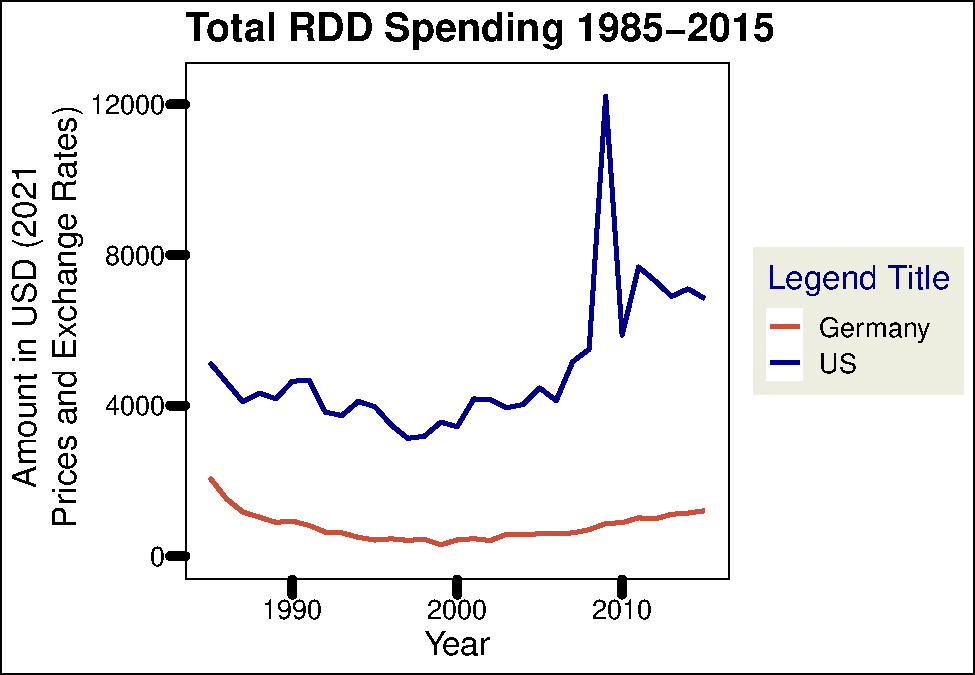
\includegraphics{Chang_Jenkins_Mullens_ENV872_Final_files/figure-latex/Germany and US Line Plot for total budget-1.pdf}
\caption{US and Germany Total RDD Spending 1985 to 2015}
\end{figure}

\begin{figure}
\centering
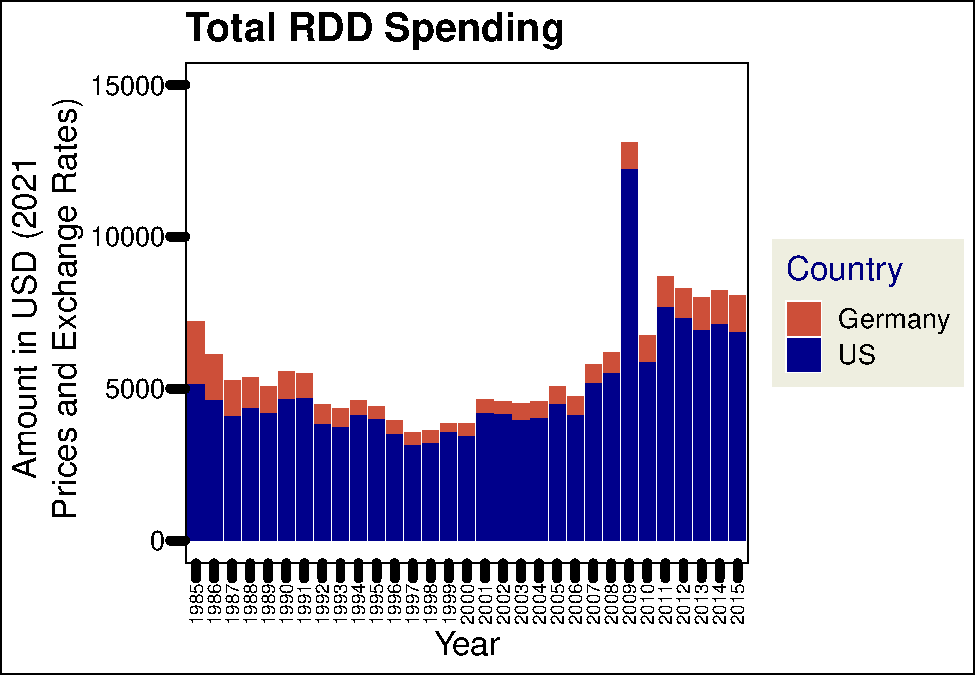
\includegraphics{Chang_Jenkins_Mullens_ENV872_Final_files/figure-latex/Germany and US Bar Plot for total budget-1.pdf}
\caption{US and Germany Total RDD Spending 1985 to 2015}
\end{figure}

\newpage

For both countries, it appears that Low Carbon RD\&D spending decreased
from 1985 to 2000 and increased from 2000 to 2015 (Figure 3).

\begin{figure}
\centering
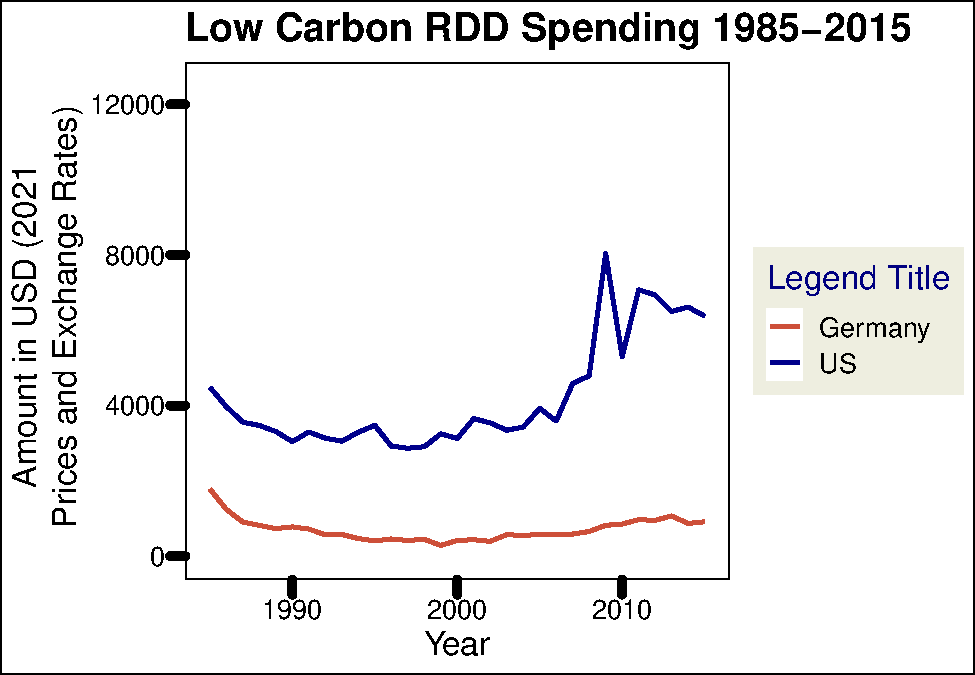
\includegraphics{Chang_Jenkins_Mullens_ENV872_Final_files/figure-latex/Low Carbon Germ and US Line Plot-1.pdf}
\caption{US and Germany Low Carbon Spending 1985 to 2015}
\end{figure}

\begin{figure}
\centering
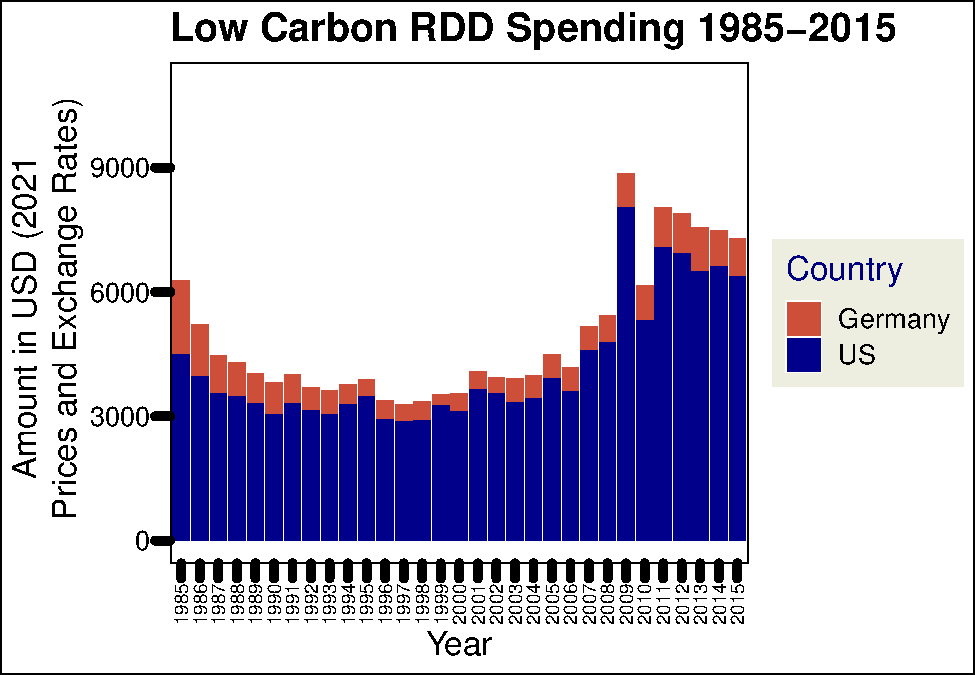
\includegraphics{Chang_Jenkins_Mullens_ENV872_Final_files/figure-latex/US and Germ Low Carbon-1.pdf}
\caption{US and Germany Low Carbon RDD Spending 1985 to 2015}
\end{figure}

\newpage

It is unclear whether these changes are significant and further analysis
is needed. A few notable abnormalities in the Germany data set include
the years 1996, 1997, and 1998 where fossil fuel spending was well below
the average (Figure 5).

\begin{figure}
\centering
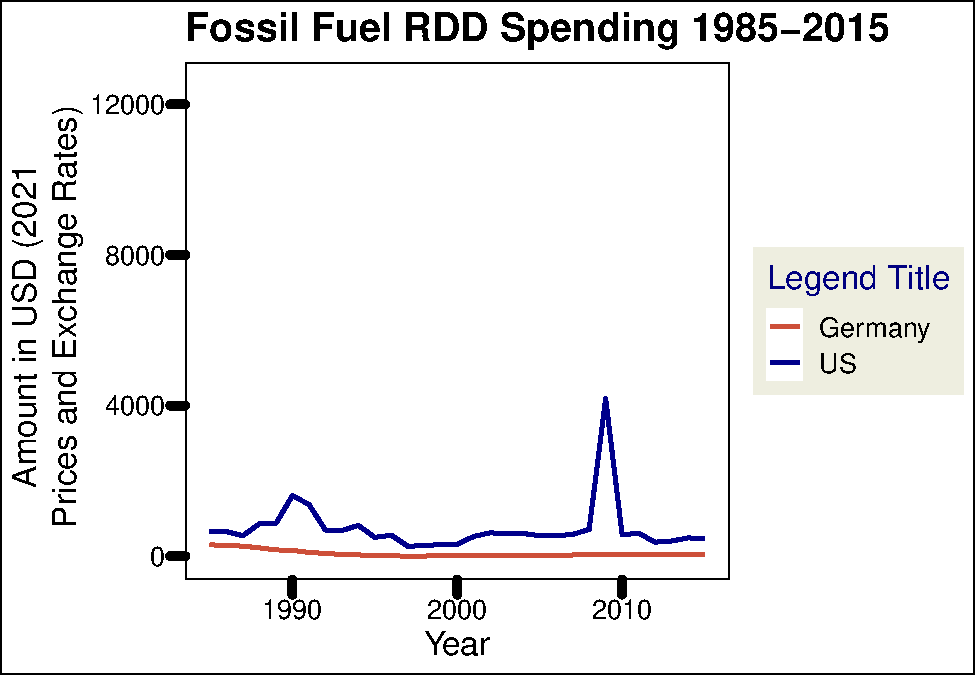
\includegraphics{Chang_Jenkins_Mullens_ENV872_Final_files/figure-latex/Fossil Fuel Germ and US Line-1.pdf}
\caption{US and Germany Fossil Fuel RDD Spending 1985 to 2015}
\end{figure}

\begin{figure}
\centering
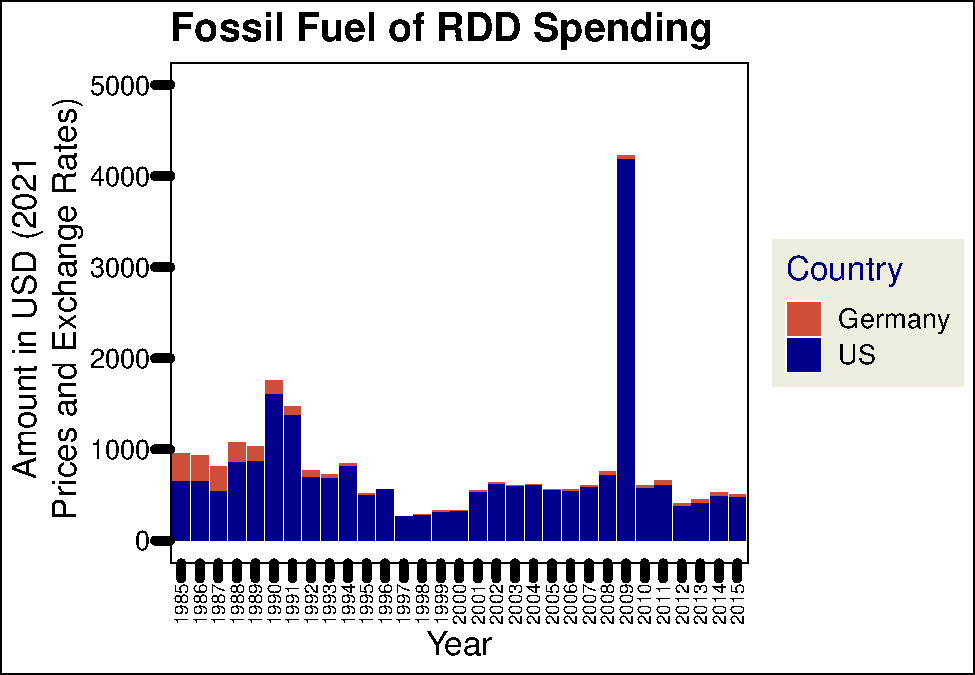
\includegraphics{Chang_Jenkins_Mullens_ENV872_Final_files/figure-latex/US and Germ fossil fuel Bar-1.pdf}
\caption{US and Germany Fossil Fuel RDD Spending 1985 to 2015}
\end{figure}

\newpage

Then, the US data was graphed alone to examine the different spending
categories, Fossil Fuels and Low Carbon Energy, against the total
spending (Figure 7). In 2009, there is a noticeable increase in the
total spending for both fossil fuels and low carbon energy; the total
budget doubled from the previous year. After the initial increase in
2009, the total budget, and consequently the low carbon energy and
fossil fuel, numbers appear to decline.

\begin{figure}
\centering
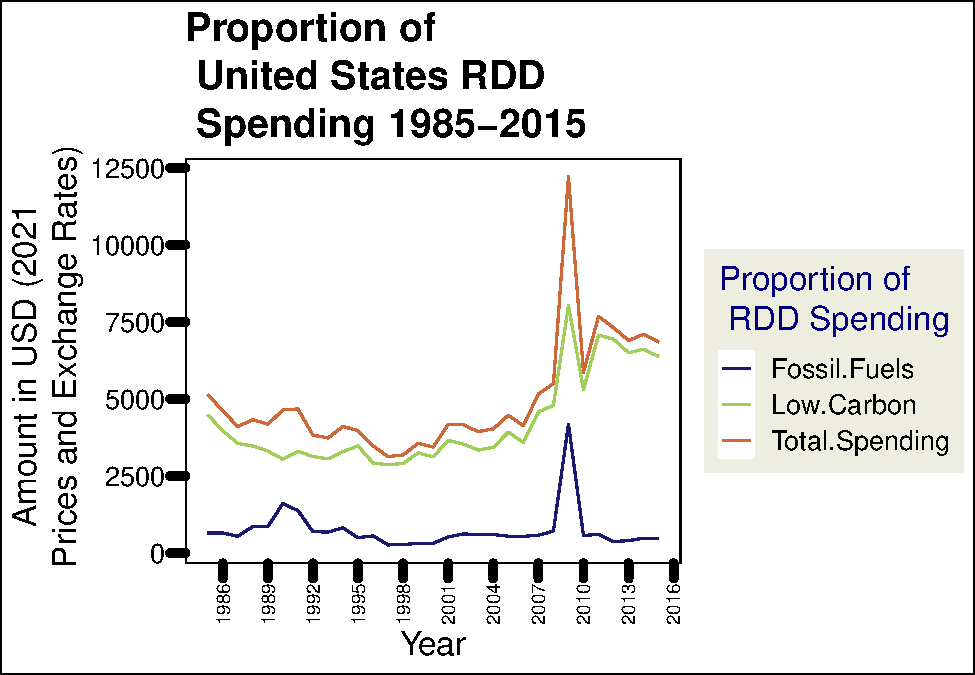
\includegraphics{Chang_Jenkins_Mullens_ENV872_Final_files/figure-latex/Line Plot of All US RDD-1.pdf}
\caption{US RDD Spending 1985 to 2015}
\end{figure}

Based on these findings, we decided two-tailed t-tests should be
administered to determine whether any changes in RD\&D during the Obama
administration were significant. It was necessary to compare the US
pre-Obama administration and the Obama administration time periods with
the RD\&D spending for Germany. However, creating a standard metric was
required to conduct this analysis. Thus, the year over year change in
RD\&D for each energy type was calculated to draw comparisons.

\newpage

\hypertarget{analysis}{%
\section{Analysis}\label{analysis}}

The analysis of the RD\&D Budget data focuses on comparing the mean
year-over-year (YoY) percent change in public low-carbon energy RD\&D
spending in the period preceding Obama's presidency (1985-2008) to the
YoY percent change during Obama's presidency (2009-2015). To ensure any
Obama-era changes in public low-carbon RD\&D investment within the
United States are unique to the administration \& its domestic energy
policy agenda, and not co-occurring with global shifts in public RD\&D
investment, trend significance in the United States was compared to the
control, Germany. To analyze these trends statistically, rather than
visually, a series of two-sample t-tests was employed using the
RDD.US.Eras data frame and filtered US.and.Germany.RDD data frame to
separately address the three research questions.

\hypertarget{united-states-pre-obama-vs.-obama-era-analysis}{%
\subsection{United States Pre-Obama vs.~Obama-era
Analysis}\label{united-states-pre-obama-vs.-obama-era-analysis}}

\textbf{Question 1:} In the United States, was the difference in means
between Pre-Obama and Obama-era year-over-year percent change in public
lower-carbon energy RD\&D spending significant?

In the first two-sample t-test, we addressed the first research question
by looking at public low-carbon energy RD\&D spending in the United
States using RDD.US.Eras data frame to determine if the mean YoY percent
change prior to Obama's presidency (1985-2008) was as significant as the
mean YoY percent change during the Obama administration (2009-2015).
RDD.US.Eras Percent.Change was the continuous dependent variable, and
RDD.US.Eras Era was the categorical variable with two levels (Pre-Obama
and Obama-era).

\begin{itemize}
\item
  \textbf{Null Hypothesis 1 (H0):} Mean YoY change in public low-carbon
  RD\&D spending during the Obama presidency (2009-2015) was not
  statistically distinct from the Pre-Obama era (1985-2008) YoY change
  in spending
\item
  \textbf{Alternative Hypothesis 1 (H1):} Mean YoY change in public
  spending on lower-carbon energy RD\&D was significantly different
  during Obama's presidency.
\end{itemize}

The test returned a p-value of 0.5771 which is above our threshold of
significance (p \textless{} 0.05). Therefore, we fail to reject our null
hypothesis (H) that mean YoY change in public low-carbon RD\&D spending
during the Obama presidency (2009-2015) was not statistically distinct
from the Pre-Obama era (1985-2008) YoY change in spending.

Figure 8 displays the year over year percent change in low carbon energy
RD\&D for both the pre-Obama and Obama time periods. A linear regression
was constructed and added to the YoY lines to examine the data trends
over time.

\newpage

\begin{verbatim}
## `geom_smooth()` using formula = 'y ~ x'
\end{verbatim}

\begin{verbatim}
## Warning: Removed 1 rows containing non-finite values (`stat_smooth()`).
\end{verbatim}

\begin{verbatim}
## `geom_smooth()` using formula = 'y ~ x'
\end{verbatim}

\begin{verbatim}
## Warning: Removed 1 row containing missing values (`geom_line()`).
\end{verbatim}

\begin{verbatim}
## Warning: Removed 1 rows containing missing values (`geom_point()`).
\end{verbatim}

\begin{figure}
\centering
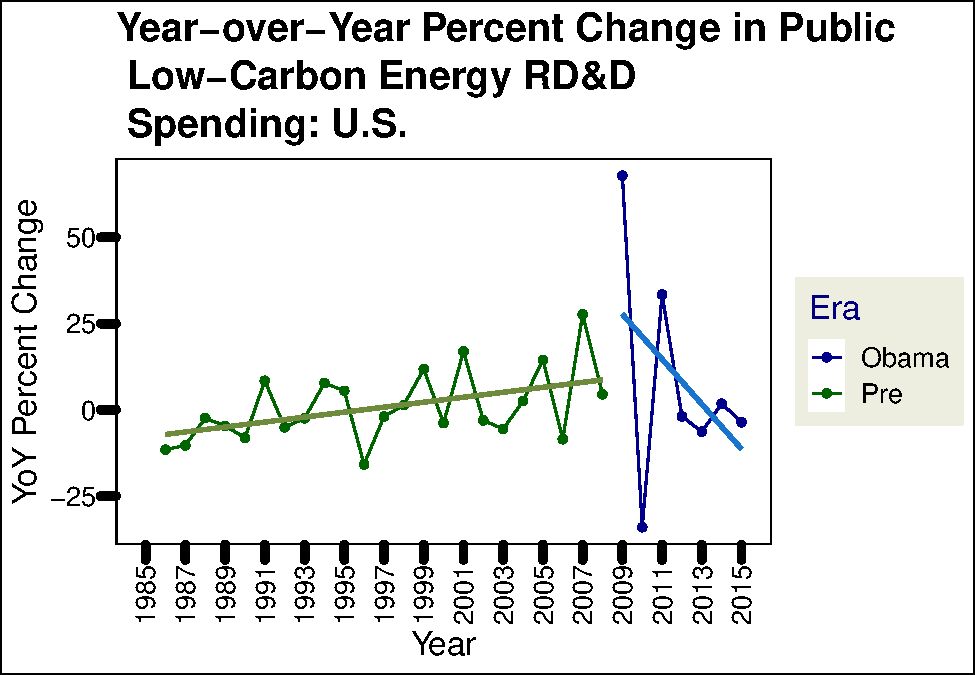
\includegraphics{Chang_Jenkins_Mullens_ENV872_Final_files/figure-latex/visualizing the US data-1.pdf}
\caption{US Year over Year RDD Spending 1985 to 2015}
\end{figure}

\hypertarget{pre-obama-united-states-vs.-germany-analysis}{%
\subsection{Pre-Obama United States vs.~Germany
Analysis}\label{pre-obama-united-states-vs.-germany-analysis}}

\textbf{Question 2:} Prior to Obama's presidency (1985-2008), was mean
year-over-year percent change in public lower-carbon energy RD\&D
spending in the United States significantly distinct from Germany?

To address the second question regarding pre-Obama spending in U.S. and
Germany, we needed to wrangle the data to only include records prior to
Obama's inauguration, for years 1985-2008. We then ran a two-sample
T-test on the filtered pre-Obama data to determine whether mean YoY
percent change in public RD\&D spending was statistically different
between the two counties. Pre.2009.US.Germany.RDD Percent.Change was the
continuous dependent variable, and Pre.2009.US.Germany.RDD Country was
the categorical variable with two levels (United States and Germany).

\begin{itemize}
\item
  \textbf{Null Hypothesis 2 (H0):} Prior to Obama's presidency, there
  was a significant difference in means between the U.S. and Germany for
  YoY percent change in public spending on lower-carbon energy RD\&D
\item
  \textbf{Alternative Hypothesis 2 (H1):} The difference in means
  between the U.S. and Germany for YoY percent change in public spending
  on lower-carbon energy RD\&D was not significant prior to Obama's
  presidency
\end{itemize}

Our test returned a p-value of 0.5113 which is above the threshold of
significance (p \textless{} 0.05). Therefore, we fail to reject the null
hypothesis (H0) that in the period prior to Obama's presidency
(1985-2008), mean year-over-year change in public low-carbon RD\&D
spending in the United States was statistically distinct from Germany.

Figure 9 displays the year over year percent change in low carbon energy
RDD for the US and Germany during the pre-Obama administration time
period. A linear regression was constructed and added to the YoY lines
to examine the data trends over time. \newpage

\begin{verbatim}
## `geom_smooth()` using formula = 'y ~ x'
\end{verbatim}

\begin{verbatim}
## Warning: Removed 1 rows containing non-finite values (`stat_smooth()`).
\end{verbatim}

\begin{verbatim}
## `geom_smooth()` using formula = 'y ~ x'
\end{verbatim}

\begin{verbatim}
## Warning: Removed 1 rows containing non-finite values (`stat_smooth()`).
\end{verbatim}

\begin{verbatim}
## Warning: Removed 2 rows containing missing values (`geom_line()`).
\end{verbatim}

\begin{verbatim}
## Warning: Removed 2 rows containing missing values (`geom_point()`).
\end{verbatim}

\begin{figure}
\centering
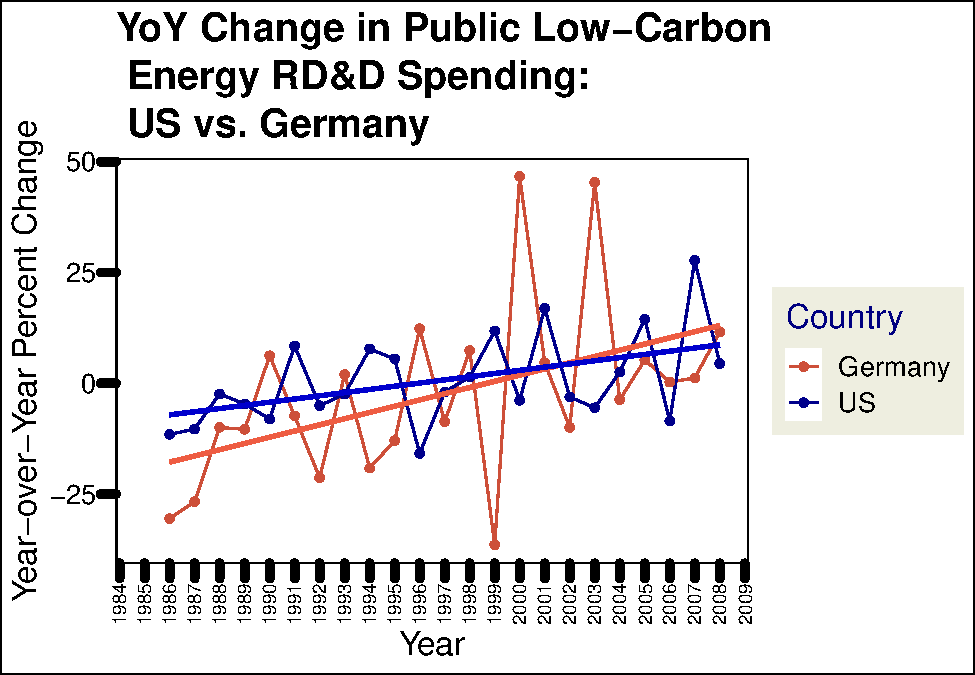
\includegraphics{Chang_Jenkins_Mullens_ENV872_Final_files/figure-latex/visualizing the pre US and Germany data together-1.pdf}
\caption{US and Germany Year over Year RDD Spending 1985 to 2008}
\end{figure}

\hypertarget{obama-era-united-states-vs.-germany-analysis}{%
\subsection{Obama-era United States vs.~Germany
Analysis}\label{obama-era-united-states-vs.-germany-analysis}}

\textbf{Question 3:} During Obama's presidency (2009-2015), was mean
year-over-year percent change in public lower-carbon energy RD\&D
spending in the United States significantly distinct from Germany?

We then conducted a similar two-sided t-test to address the third
question regarding Obama-era spending in the U.S. and Germany. After
wrangling the data to only include records during Obama's two-term
presidency, for years 2009-2015, we ran the analysis on the filtered
data to determine whether mean YoY percent change in Obama-era public
RD\&D spending was statistically different between the two counties.
Post.2009.US.Germany.RDD Percent.Change was the continuous dependent
variable, and Post.2009.US.Germany.RDD Country was the categorical
variable with two levels (United States and Germany).

\begin{itemize}
\item
  \textbf{Null Hypothesis 3 (H0):} During Obama's presidency, mean YoY
  percent change in public spending on lower-carbon energy RD\&D in the
  United States was not statistically distinct from Germany YoY change
  in spending
\item
  \textbf{Alternative Hypothesis 3 (H1):} Obama-era YoY percent change
  in public lower-carbon energy RD\&D spending in the United States was
  significantly different from Germany YoY change in spending
\end{itemize}

The final two-sided t-test returned a p-value of 0.857 which is above
the threshold of significance (p \textless{} 0.05). Therefore, we fail
to reject the null hypothesis (H0) that mean YoY change in public
low-carbon RD\&D spending in the U.S. was not statistically distinct
from Germany during the Obama Administration.

Figure 10 displays the year over year percent change in low carbon
energy RDD for the US and Germany during the Obama administration time
period. A linear regression was constructed and added to the YoY lines
to examine the data trends over time.

\newpage

\begin{verbatim}
## `geom_smooth()` using formula = 'y ~ x'
## `geom_smooth()` using formula = 'y ~ x'
\end{verbatim}

\begin{figure}
\centering
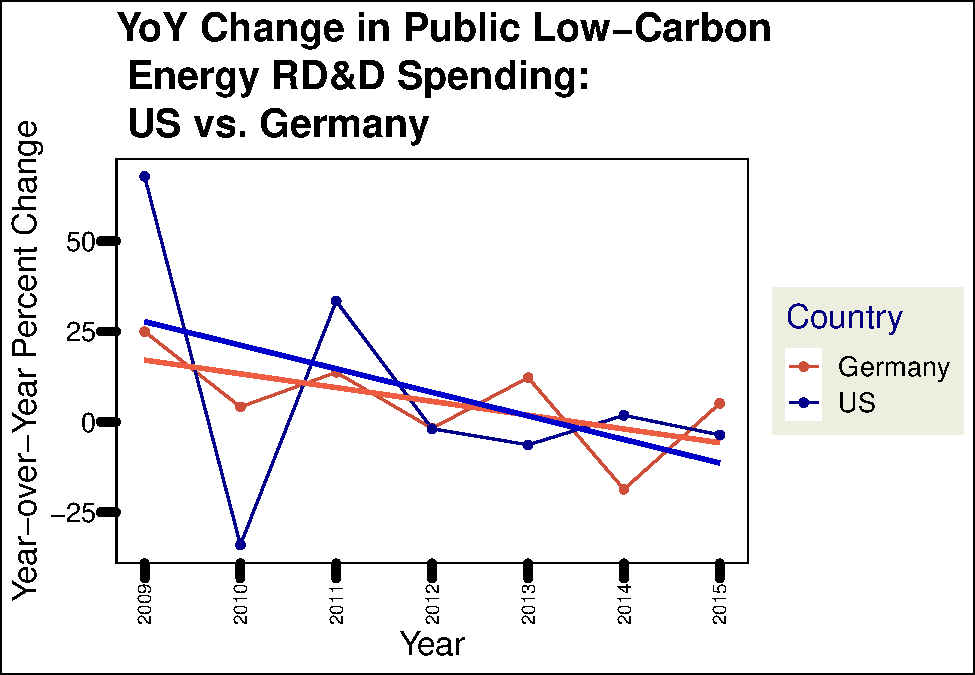
\includegraphics{Chang_Jenkins_Mullens_ENV872_Final_files/figure-latex/visualizing Obama US and Germany data together-1.pdf}
\caption{US and Germany Year over Year RDD Spending 2009 to 2015}
\end{figure}

\newpage

\hypertarget{summary-and-conclusions}{%
\section{Summary and Conclusions}\label{summary-and-conclusions}}

\textbf{List of p-values from two-sided t-test analyses.}

\begin{longtable}[]{@{}ll@{}}
\toprule()
Analysis & p\_value \\
\midrule()
\endhead
US.PreObama.v.ObamaEra & 0.5771 \\
PreObama.US.v.Germany & 0.5113 \\
ObamaEra.US.v.Germany & 0.857 \\
\bottomrule()
\end{longtable}

The results from the two-sided t-tests, which indicated non-significant
differences in mean YoY percent change in public low-carbon energy RD\&D
spending between different time periods and between the United States
and Germany, were unexpected and contrary to the initial hypotheses. The
initial exploration of relationships using the raw budget data for both
the United States and Germany suggested a significant distinction in
U.S. lower-carbon energy RD\&D spending at the onset of Obama's two-term
presidency.

Regarding findings from the analysis of the first research question, the
insignificant difference in mean YoY percent change in public
lower-carbon energy RD\&D spending between the pre-Obama and Obama-era
periods does not necessarily suggest that a substantial shift in funding
priorities or levels of investment did not occur during Obama's
presidency. The unexpected result (p-value = 0.5771), and failure to
reject the null hypothesis, might be explained by the selection of the
continuous dependent variable, mean year-over-year percent change in
public lower-carbon energy RD\&D spending. After visualizing
relationships in the raw data -- particularly the substantial low-carbon
energy RDD budgetary swings starting in Obama's first year in office --
statistical analysis focused on the average YoY percent change in
spending. While this approach captures the overall direction \&
magnitude of change in RD\&D spending, it smooths out short-term
fluctuations over the selected time period and presents a less
pronounced view of the trends. Thus, the analysis of the mean YoY
percent change offset the potentially significant fluctuations that were
initially explored rather than emphasizing specific annual variations in
Obama's first years in office. Regardless, the low-carbon energy policy
wins, particularly within Obama's first term, that underlay the original
rationale affirm that it was a pivotal moment in the United States'
transition towards renewable energy.

Similarly, regarding the second and third research questions, the
non-significant difference in mean YoY percent change in public
lower-carbon energy RD\&D spending between the U.S. and Germany during
both the pre-Obama (p-value of 0.5113) and Obama-era (p-value = 0.857)
time periods contradicts the initial expectations. Failing to reject the
null hypotheses, these findings indicate that the two countries had
similar public investment trends in clean energy technologies,
suggesting that factors other than the Obama Administration's policy
interventions may have influenced changes in low-carbon RD\&D spending.
Again, despite the divergent trends observed in the analysis, landmark
policy such as the 2009 American Recovery and Reinvestment Act helps
validate the original rationale and hypotheses that the Obama
Administration marked a notable shift in sustainable energy funding
priorities and investment levels.

The unexpected findings from these analyses underscores the importance
of further exploration to understand the underlying factors driving
RD\&D spending in the United States and Germany. To gain a more
comprehensive understanding of the significance of low-carbon RD\&D
spending during Obama's two-term presidency, it would be beneficial to
uncouple financial spending from environmental impact. While there was
not a significant increase in low carbon energy investments during the
Obama administration, this does not mean that there was not a
significant change in environmental impact, such as a potential decrease
in greenhouse gas emissions resulting from increased spending through
the 2009 Recovery Act. Therefore, further literature review and research
on the environmental impact stemming from increased funding through the
Department of Energy may be beneficial to understanding the full
magnitude the Obama Administration had on the transition towards lower
carbon energy through RD\&D investment.

\newpage

\#Scripts, data and code The repository linked at the beginning contains
both the raw data, wrangled data, and code utilized. They are found in
their respective folders.

\#Quality assurance Please note that any conclusions created by this
report are limited as only one source of data and one variable were
utilized. Further examination of additional metrics and countries are
recommended for future analyses.

\newpage

\hypertarget{references}{%
\section{References}\label{references}}

Energy Technology RD\&D Budgets. (2023, April). International Energy
Agency. Retrieved April 1, 2023 from
\url{https://www.iea.org/data-and-statistics/data-product/energy-technology-rd-and-d-budget-database-2}

Office of Electricity. (n.d.). 2009 American Recovery and Reinvestment
Act. U.S. Department of Energy. Retrieved May 2, 2023, from
\url{https://www.energy.gov/oe/2009-american-recovery-and-reinvestment-act}.

\textless add references here if relevant, otherwise delete this
section\textgreater{}

\end{document}
